\definecolor{exxetagray}{gray}{0.75}
\definecolor{itemcolor}{RGB}{179,217,255}
\definecolor{usercolor}{RGB}{255,204,179}

\shorthandoff{"}
\chapter{Verwandte Arbeiten}
\label{ch:verwandte_arbeiten}
In der Literatur existieren bereits diverse Veröffentlichungen, die sich mit der Berücksichtigung wechselseitiger Präferenzen für die automatische Zuweisung von Personen für Jobpositionen beschäftigen.
Während einige Veröffentlichungen Reziprozität als multi-kriterielles Problem betrachten, ordnen andere Arbeiten die reziproke Empfehlungserstellung nicht explizit als multi-kriterielles Problem ein.
Dadurch haben sich im Verlauf der Jahre unterschiedliche Ansätze für die Berücksichtigung wechselseitiger Präferenzen von Nutzern und Elementen in Empfehlungssystemen entwickelt.
% Auch wenn der Fokus eines Großteils der Veröffentlichungen auf der Vorhersage wechselseitiiger Empfehlungen beruht, lassen sich dennoch Ansätze für die Integration bilateraler Präferenzen in Empfehlungssysteme unterscheiden.
% Nachfolgend werden verwandte Arbeiten zu reziproken Empfehlungssystemen mit Bezug auf die vorliegende Domäne angeführt.

\section{Nicht als multi-kriteriell bezeichnete wechselseitige Systeme}
% Gemäß \textcite[S. 1467]{yildirim:article} hat die wechselseitige Empfehlung in der Literatur bis heute wenig Aufmerksamkeit erhalten.
% Dies begründen \textcite[S. 1467]{yildirim:article} durch eine begrenzte Verfügbarkeit öffenlticher Datensätze mit Angaben zu Präferenzen der Nutzer eines Netzwerks.

Die erste Veröffentlichung in der Literatur zu wechselseitigen Empfehlungssystemen stammt von \textcite[S. 1ff.]{pizzato:inproceedings}, welche ein wechselseitiges Empfehlungssystem für Online-Dating-Plattformen vorstellen \cite[S. 1469]{yildirim:article}.
Nach \textcite[S. 5]{pizzato:inproceedings} ergibt sich der Wert einer \ac{N-E-K} grundsätzlich aus einer Kombination der Präferenz eines Nutzers für ein Element und der Präferenz eines Elements für einen Nutzer.
Die Autoren weisen darauf hin, dass für die Kombination der beiden Komponenten verschiedene Methoden verwendet werden können.
In ihrer Veröffentlichung modellieren \textcite[S. 6]{pizzato:inproceedings} eine reziproke Empfehlung als gewichtete Summe aus dem Wert der Präferenz eines Nutzers für ein Element ($P1$) und dem Wert der Präferenz eines Elements für einen Nutzer ($P2$) \cite[S. 6]{pizzato:inproceedings}:
\begin{equation}\label{eq32}
    PRR(c,s) = w_{1}P1(c,s) + w_{2}P2(c,s)
\end{equation}
Über die Gewichte $w_{1}$ und $w_{2}$ können die Präferenzen von Nutzern bzw. Elementen unterschiedlich gewichtet werden \cite[S. 6]{pizzato:inproceedings}.
Für alternative Kombinationsmöglichkeiten der bilateralen Präferenzen verweisen \textcite[S. 5]{pizzato:inproceedings} auf \textcite[S. 339ff.]{burke:article}, der in seiner Veröffentlichung zu hybriden Empfehlungssystemen allgemeine Methoden für die Kombination von Ergebnissen unterschiedlicher Systeme vorstellt.
Auch wenn die Umsetzung der reziproken Empfehlung bereits als multi-kriterieller Ansatz modelliert wurde (Vgl. Gleichung \ref{eq32}), bezeichnen \textcite[S. 1ff.]{pizzato:inproceedings} die wechselseitige Empfehlungserstellung nicht ausdrücklich als multi-kriterielles Problem. 

Eine Umsetzung des Konzepts wechselseitiger Empfehlungssysteme stellen \textcite[S. 207ff.]{pizzato:2010} in einer weiterführenden Arbeit vor.
Die Autoren entwickeln einen inhaltsbasierten Algorithmus für eine Online-Dating-Website, welche die bilateralen Präferenzen zweier Nutzer $x$ und $y$ über das harmonische Mittel aggregiert:
\begin{equation}\label{eq33}
    PRR(x,y) = \frac{2}{(\frac{1}{Comp.(P_{x,y})}+\frac{1}{Comp.(P_{y,x})})}
\end{equation}
Als Indikator für die Präferenzen $P_{x}$ eines Nutzers $x$ stützen sich die Autoren auf Attribute der Nutzer, die eine Nachricht des Nutzers $x$ erhalten haben.
So gehen \textcite[S. 210]{pizzato:2010} davon aus, dass ein Nutzer $x$ eine bestimmte Altersgruppe bevorzugt, wenn er im Vergleich zu anderen Altersgruppen maßgeblich Nutzern einer Altersklasse Nachrichten gesendet hat.
Die Präferenz eines Nutzers $x$ für einen Nutzer $y$ bestimmen \textcite[S. 210]{pizzato:2010} über einen Komnpatibilitäs-Wert $Comp.(P_{x,y})$, der sich aus der Präferenz des Nutzers $x$ für die Attribute des Nutzers $y$ ergibt.
Bis heute wird davon ausgegangen, dass die meisten der später vorgeschlagenen Modelle zu \ac{RRS} auf dem Ansatz von \textcite[S. 207ff.]{pizzato:2010} basieren \cite[S. 723]{kumari:article}.

% Negative Präferenzen? s.u.

Kritisch ist anzumerken, dass die Präferenzen der Nutzer in der Ermittlung des reziproken Wertes nicht unterschiedlich stark gewichtet werden können.
Demzufolge ist der reziproke Wert eines Nutzers $x$ für einen Nutzer $y$ symmetrisch zu dem Wert eines Nutzers $y$ für einen Nutzer $x$ \cite[S. 211]{pizzato:2010}.
% Darüber hinaus weisen \textcite[S. 285]{zheng:2:inproceedings} darauf hin, dass eine unterschiedliche Gewichtung notwendig sein kann, bspw. wenn die Kompatibilitätswerte auf unterschiedlichen Skalen oder Verteilungen liegen.
Weiter ist eine Voraussetzung für die Bestimmung des Wertes bilateraler Präferenzen anhand des harmonischen Mittels, dass die jeweiligen Kompatibilitätswerte nicht null sein dürfen, da das harmonische Mittel für solche Werte nicht definiert ist.
Dies muss beim Aufsetzen des Algorithmus berücksichtigt werden.
% Vorstellung ergebnisse des Algorithmus?

\textcite[S. 40]{li:inproceedings} bemängeln an dem Ansatz von \textcite[S. 207ff.]{pizzato:2010}, dass wesentliche Charakteristika wechselseitiger Empfehlungssysteme außer Acht gelassen werden.
Sie merken an, dass Aspekte wie Passivität und die Endlichkeit von Nutzern nicht in die Empfehlungserstellung miteinbezogen werden.
Zusätzlich zu der Berücksichtigung weiterer Aspekte wechselseitier Empfehlungssysteme, wird der Wert der Reziprozität in dem allgemeinen Framework für \ac{RRS} von \textcite[S. 38]{li:inproceedings} als Produkt der Präferenzwerte zweier Nutzer $x$ und $y$ bestimmt \cite[S. 710]{kumari:article}.
Den Autoren zufolge soll dadurch eine unilaterale Präferenz im Vergleich zu herkömmlichen Aggregationsmethoden (z.B. Linearkombination) verhindert werden.
Dies betrifft beispielsweise Fälle in denen lediglich eine Person den Präferenzen der anderen Person entspricht, zum Beispiel in Fällen in denen ein Bewerber eine Jobposition bevorzugt, dieser aber nicht für die ausgeschriebenen Stelle geeignet ist \cite[S. 38]{li:inproceedings}.

\textcite[S. 66ff.]{diaz:inproceedings} formulieren das Finden optimaler Paare in Online-Dating-Plattformen als Informationsbeschaffungsproblem\footnote{"Information retrieval problem" - \textcite[S. 67]{diaz:inproceedings}} \cite[S. 550]{koprinska:inbook}.
\textcite[S. 550]{koprinska:inbook} beschreiben die Veröffentlichung der Autoren als einen Ansatz für das Ranking von Nutzern in Abhängighkeit ihrer Übereinstimmung mit dem idealen Partnerprofil eines Nutzers (d.h. Ausprägungen strukturierter und unstrukturierter Profilattribute \cite[S. 288]{li:article}\cite[S. 272]{pizzato:2:inproceedings}).
Die Autoren verwenden historische Daten, mithilfe derer Paare von Nutzern als "relevant" bzw. "nicht-relevant" gekennzeichnet werden.
Als relevant bezeichnen die Autoren Paare, in denen Nutzer Kontaktinformation ausgetauscht haben \cite[S. 66ff.]{diaz:inproceedings}.
Unter Verwendung eines Gradient Boosted Decision Trees (Machine-Learning Technik) und den gekennzeichneten historischen Daten ermitteln \textcite[S. 69]{diaz:inproceedings} die angenommene Relevanz potenzieller Kandidaten für einen Nutzer \cite[S. 550]{koprinska:inbook}.
Die Ermittlung des Verlusts in dem Machine-Learning Modell von \textcite[S. 69]{diaz:inproceedings} erfolgt durch Anwendung der mittleren quadratischen Abweichung (engl.: \ac{MSE}).
Den Aspekt der Reziprozität bezeichnen \textcite[S. 66]{diaz:inproceedings} als two-sided relevance (dt.: zweiseitige Relevanz) \cite[S. 550]{koprinska:inbook}.

\textcite[S. 247ff.]{kim:2:inproceedings} entwickelten eine Methode für die bilaterale Empfehlungserstellung in sozialen Netzwerken.
In ihrer Arbeit beziehen sich die Autoren auf Netzwerke, in denen Nutzer auf Nachrichten anderer Nutzer positiv bzw. negativ reagieren können \cite[S. 548]{koprinska:inbook} .
Der Ansatz von \textcite[S. 247ff.]{kim:2:inproceedings} berücksichtigt für die Empfehlungserstellung sowohl die Interessen des Senders einer Nachricht, als auch die Interessen des Empfängers einer Nachricht.
Ähnlich zu dem Ansatz von \textcite[S. 207ff.]{pizzato:2010} erfolgt die Aggregation durch Verwendung des gewichteten harmonischen Mittels \cite[S. 251]{kim:2:inproceedings}.
Dies ermöglicht eine unterschiedliche Gewichtung des Interesses $I$ von Sender $x$ an Empfänger $y$ bzw. von Empfänger $y$ an Sender $x$ über die Parameter $w_{x}$ und $w_{y}$ \cite[S. 251]{kim:2:inproceedings}:
\begin{equation}\label{eq34}
    H(x,y) = \frac{2}{(\frac{w_{x}}{I_{x,y}}+\frac{w_{y}}{I_{y,x}})}
\end{equation}
Anküpfende Experimente von \textcite[S. 259]{kim:2:inproceedings} zeigen nur eine geringe Schwangung des Anteils positiver Interaktionen von Empfängern am Gesamtaufkommen der Interaktionen in Abhängigkeit der gewählten Gewichte für die Interessen.
Die Autoren gehen davon aus, dass die geringe Schwankung maßgeblich aufgrund des retrospektiven Charakters der historischen Daten besteht \cite[S. 259]{kim:2:inproceedings}.
Die Veröffentlichung von \textcite[S. 259]{kim:2:inproceedings} kann folglich keine Aussage darüber treffen, wie Nutzer auf Empfehlungen reagieren, die anhand unterschiedlicher Gewichte ermittelt wurden.
% Dies ist durch die Art der Ermittlung des Interesses eines Empfängers zu erklären, welches durch das Verhältnis von positiven Rückmeldungen eines Empfängers zu allen Interaktionen eines Senders bemessen wird.
% Da die Anzahl an Rückmeldungen bereits in der Vergangenheit ermittelt wurde, hat eine höhere Gewichtung dieser keinen Einfluss auf vergangene Interaktionen, lediglich auf die Ermittlung des harmonischen Mittels.

\textcite[S. 131ff.]{kleinerman:2:inproceedings} stellen fest, dass in \ac{RRS} bislang offen blieb, wie die unilateralen Präferenzen zweier Parteien optimal im Gleichgewicht gehalten werden können.
Die Autoren entwickelten daher eine Methode (sog. \ac{RWS}) für Online-Dating-Plattformen, die Empfehlungen basierend auf dem optimalen Gleichgewicht zwischen den Interessen zweier Personen erstellt.
Im Vergleich zu vorherigen Ansätzen, in denen für alle Nutzer die Präferenzen beider Parteien gleichermaßen in den reziproken Wert einflossen, erfolgt die Gewichtung mit \ac{RWS} für jeden Nutzer individuell, basierend auf dessen vergangenen Interaktionen \cite[S. 133]{kleinerman:2:inproceedings}.
\ac{RWS} kombiniert für jeden Nutzer $c$ die Wahrhscheinlichkeit, dass dieser Interesse an einer empfohlenen Person $c'$ aufweist ($CF_{c,c'}$) und die Wahrscheinlichkeit, dass die empfohlene Person $c'$ dies positiv erwidert ($PR_{c',c}$) \cite[S. 131f.]{kleinerman:2:inproceedings}:
\begin{equation}\label{eq36}
    RWS_{c,c'}(\alpha_{c}) = \alpha_{c} \cdot CF_{c,c'} + (1-\alpha_{c}) \cdot PR_{c',c}
\end{equation}
Der Parameter $\alpha$ wird anhand des Einflusses der einzelnen Werte ($CF$ und $PR$) auf erfolgreiche Interaktionen des Nutzers $x$ aus der Vergangenheit ermittelt \cite[S. 135]{kleinerman:2:inproceedings}.
Für die Vorhersage der Interessen von $c$ verwenden die Autoren kollaboratives Filtern, während für die Vorhersage der Rückmeldung durch $c'$ Techniken des Maschinellen Lernens verwendet werden.
Die \ac{RWS} von \textcite[S. 134]{kleinerman:2:inproceedings} ist nachfolgend in Abbildung \ref{fig:relatedwork:abb2} anhand eines Beispiel-Nutzers grafisch dargestellt.

\begin{figure}[H]
    \centering
	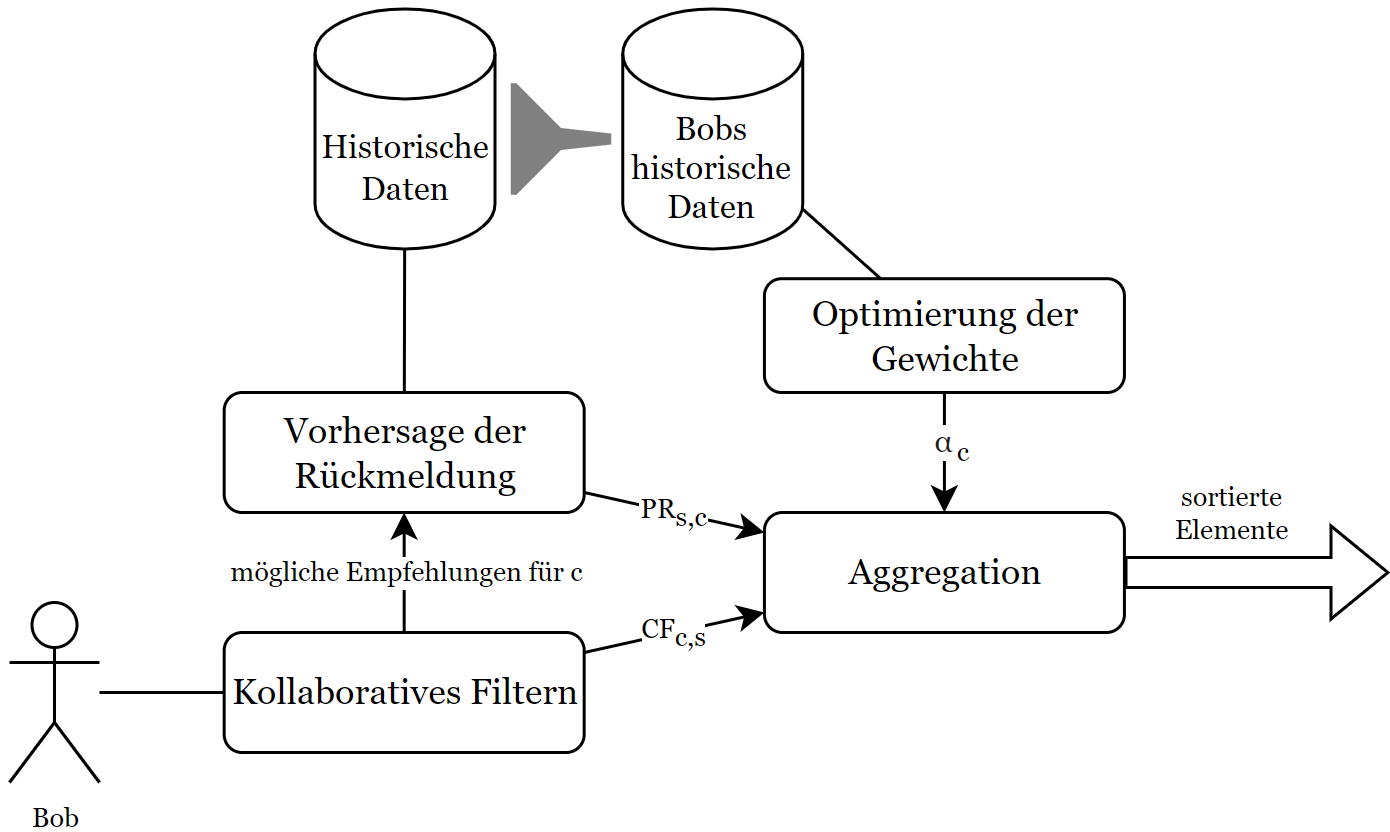
\includegraphics[width=0.9\textwidth]{gfx/rws.png}
	\caption[Reciprocal Weighted Score]{Reciprocal Weighted Score\\
    (Eigene Darstellung in Anlehnung an \cite[S. 134]{kleinerman:2:inproceedings})}
	\label{fig:relatedwork:abb2}
\end{figure}

Um für Nutzer ohne erfolgreiche Interaktionen in der Vergangenheit Empfehlungen zu erstellen, definieren die Autoren zusätzlich ein Optimierungsproblem über alle Nutzer eines Systems hinweg \cite[S. 135]{kleinerman:2:inproceedings}:
\begin{equation}\label{eq37}
    \begin{aligned}
        \min_{\alpha} \sum_{c \in C} \sum_{c' \in V_{c}} \mathbb{1}_{c' \in SuccInter_{c}} Rank_{c'} (RWS_{c,*}(\alpha))\\
        \textnormal{u.d.B. } 0 \geq \alpha \geq 1\\
    \end{aligned}
\end{equation}
Hierbei stellt $V_{c}$ die Menge aller Personen $c'$ dar, deren Profil $c$ betrachtet hat und $\mathbb{1}_{c' \in SuccInter_{c}}$ eine Indikatorfunktion, welche $1$ ausgibt, wenn eine Person $c'$ eine erfolgreiche Interaktion mit $c$ aufweist und $0$ andernfalls.
$Rank_{c'} (RWS_{c,*}(\alpha))$ gibt den Rang einer Person $c' \in V_{c}$ im Ranking für einen Nutzer $c$ an \cite[S. 135]{kleinerman:2:inproceedings}.
Für die Lösung des Optimierungsproblems verwenden die Autoren den Algorithmus von \textcite[S. 422ff.]{brent:article} für die lokale Minimumsuche innerhalb eines angegebenen Intervalls.
Aus der Lösung resultiert das Gewicht $\alpha$, welches Personen, die erfolgreiche Interaktionen mit einem Nutzer aufweisen, höher im Ranking platziert \cite[S. 135]{kleinerman:2:inproceedings}.

In anknüpfenden Experimenten untersuchten die Autoren die Bedeutung der individuellen Gewichtung in Online-Dating-Plattformen.
Hierfür verglichen sie ihren Ansatz mit einer bekannten Methode für wechselseitige Empfehlungssysteme von \textcite[S. 6]{xia:inproceedings}, welche die Interessen der Nutzer über das harmonische Mittel aggregiert.
Dabei stellten die Autoren fest, dass durch die gewichtete Methode die Anzahl erfolgreicher Interaktionen im Vergleich zum Benchmark gesteigert werden konnte \cite[S. 132]{kleinerman:2:inproceedings}.
Gleichzeitig führte die Methode jedoch zu einer Abnahme der relevanten Vorschläge für einen Nutzer.
Dies begründen \textcite[S. 132]{kleinerman:2:inproceedings} damit, dass ihn ihren Experimenten im Durchschnitt das Interesse der empfohlenen Personen (d.h. $PR$) stärker gewichtet wurde.
Darüber hinaus kritisieren die Autoren an ihrer Methode, dass die Optimierung auf Individuen-Level zu einer erhöhten Laufzeit führt.
Eine Reduktion der Laufzeit sei durch Verlagerung der Ermittlung der Gewichte in eine Offline-Phase denkbar \cite[S. 138]{kleinerman:2:inproceedings}.
Grundsätzlich gehen  \textcite[S. 138]{kleinerman:2:inproceedings} davon aus, dass ihr Ansatz auch für verwandte Domänen wie dem Online-Recruitment von Relevanz ist.

Im Vergleich zu verwandten Domänen hat die automatische Zuordnung von Personen zu Jobpositionen in der Literatur bislang wenig Aufmerksamkeit erhalten \cite[S. 1469]{yildirim:article}.

\textcite[S. 1ff.]{malinowski:2006} stellen in ihrer Arbeit die Notwendigkeit der Berücksichtigung bilateraler Präferenzen für die Zuordnung von Personen zu Jobpositionen fest.
Die Autoren führen den Begriff des \ac{P-E Fit} ein, welcher häufig in der Berufs- und Organisationspsychologie Anwendung findet \cite[S. 2]{link:booklet} und eine optimale Zuordnung einer Person zu ihrer Umgebung beschreibt.
Gemäß \textcite[S. 1ff.]{malinowski:2006} hängt eine optimale Zuordnung von Person zu Arbeitsumgebung (d.h. \ac{P-E Fit}) von vier Komponenten ab: dem Person-Job-Fit, dem Person-Oganisation-Fit, dem Per\-son-Vocation-Fit und dem Person-Group-Fit \cite[S. 3]{malinowski:2006}.
Diese Zuordnung kann signifikante Auswirkungen (z.B. Zufriedenheit, Leistung, Stress) haben \cite[S. 83]{su:2015}.
In ihrer Arbeit fokussieren sich \textcite[S. 4]{malinowski:2006} auf die optimale Zuordnung von Person zu Job (Person-Job-Fit).
Sie stellen fest, dass für die reziproke Empfehlungerstellung die Bedürfnisse der Recruiter und die Bedürfnisse der Bewerber zu einem Indikator \cite[S. 922]{siting:2012} aggregiert werden müssen \cite[S. 5]{malinowski:2006}.
Die Bestimmung einer optimalen Zuordnung als Kombination aus den Bedürfnissen der Recruiter und den Bedürfnissen der Bewerber definieren die Autoren als Problem des Findens einer pareto-optimalen Lösung \cite[S. 5]{malinowski:2006}.
Jedoch führten \textcite[S. 1ff.]{malinowski:2006} keine Implementierung und Evaluation einer solchen Kombination durch \cite[S. 549]{koprinska:inbook}.
% HIER KRITIK NENNEN VON RECON!

Eine erste Implementierung und Evaluation eines bilateralen Ansatzes für die Zuordnung von Personen zu Projektpositionen stellt \textcite[S. 1ff.]{link:booklet} vor.
In seiner Arbeit führt \textcite[S. 2]{link:booklet} an, dass bislang keine Publikation belegt, dass eine Zuordnung von Mitarbeitern zu Projektpositionen durch ein wechselseitiges Empfehlungssystem die Theorie des \ac{P-E Fit} und die damit verbundenen Auswirkungen erzielen kann.
Daher entwickelte \textcite[S. 1ff.]{link:booklet} ein Empfehlungssystem, das Mitarbeiter sowohl ausschließlich anhand der Präferenzen von Projektmanagern (unilateral) als auch unter Einbezug der Präferenzen der Mitarbeiter (bilateral) sortiert.
In seiner Arbeit evaluiert der Autor, ob der bilaterale Ansatz die Zufriedenheit der Mitarbeiter sowie die erwartete Arbeitsleistung dieser seitens der Projektmanager im Vergleich zu dem unilateralen Ansatz steigert.
Für die Abbildung der Präferenz eines Mitarbeiters für eine Projektposition verwendet das System boolesche Werte \cite[S. 69]{link:booklet}.
Die Berücksichtigung der Präferenzen der Mitarbeiter erfolgt, indem das System für einen Mitarbeiter, der eine Projektposition präferiert, die höchste Bewertung dieser Fähigkeit innerhalb des Kompetenzniveaus des Angestellten zu dessen Beurteilung addiert \cite[S. 44]{link:booklet}.
\textcite[S. 44]{link:booklet} begründet diese Aggregation der Präferenzen damit, dass die ursprüngliche Reihenfolge der Mitarbeiter bestehen bleibt und Projektmanager zugleich den fähigsten und motiviertesten Angestellten vorgeschlagen bekommen.

Kritisch ist anzumerken, dass diese Methode keine durchgängige Gewichtung der Präferenzen von Mitarbeitern vorsieht.
Dies führt zwangsläufig dazu, dass alle Mitarbeiter innerhalb einer Kompetenzstufe einer Fähigkeit, die diese Fähigkeit präferieren, höher eingestuft werden als der fähigste Mitarbeiter dieser Kompetenzstufe, der keine Präferenz angegeben hat.
Da der Einfluss der Präferenz eines Mitarbeiters auf das jeweilige Kompetenzniveau begrenzt ist, verhindert \textcite[S. 1ff.]{link:booklet}, dass Mitarbeiter mit geringen Kenntnissen in einer Fähigkeit durch Präferenz höher gelistet werden als Mitarbeiter mit Expertenwissen.
Dies macht es jedoch zugleich unmöglich, dass Mitarbeiter mit Kenntnissen am oberen Rand eines Kompetenzniveaus einer Fähigkeit, die diese Fähigkeit präferieren, höher gelistet werden, als Mitarbeiter mit Kenntnissen am unteren Rand der angrenzenden Kompetenzstufe, die diese Fähigkeit nicht präferieren.

Des weiteren bemängelt \textcite[S. 69]{link:booklet}, dass aus einer fehlenden Angabe zu der Präferenz eines Mitarbeiters für eine Projektposition nicht hervorgeht, ob dieser einer Fähigkeit neutral gegenübersteht, oder diese nicht bei zukünftigen Projektarbeiten anwenden möchte.

\section{Als multi-kriteriell bezeichnete wechselseitige Systeme}
% Obwohl \ac{MCDA} in der Literatur im Bereich Operations Research bereits intensiv behandelt wurde \cite[S. 220]{lakiotaki:inproceedings}, merken \textcite[S. 248]{kim:2:inproceedings} an, dass die Thematik in dem Kontext von Empfehlungssytemen bislang wenig Aufmerksamkeit erhalten hat.

% Wie in Kapitel \ref{ch:erweiterungen:bedeutung} angeführt, werden Techniken der \ac{MCDA} in Empfehlungssystemen größtenteils angewandt, um multi-kriterielle Bewertungen in der Vorhersage fehlender \ac{N-E-K} einzusetzen.
% So ermitteln \textcite[S. 48ff.]{adomavicius:inproceedings:2} und \textcite[S. 235ff.]{jhalani:inproceedings} unbekannte Bewertungen für Filme des Yahoo!Movie-Datensatzes über kollaboratives Filtern auf Kriterien-Ebene und nutzen Lineare Regression, um basierend auf vergangenen Bewertungen die Gewichte einzelner Kriterien für Nutzer zu ermitteln (nutzerbasierte Aggregationsfunktion).
% \textcite[S. 2456]{zheng:inproceedings} und \textcite[S. 678]{jannach:2:article} verwenden ebenfalls kollaboratives Filtern für die Vorhersage multi-kriterieller Bewertungen, jedoch wird \ac{SVR} für das Lernen der individuellen Gewichte von Nutzern und Elementen angewandt.
% Den Einsatz von \ac{SVR} begründen die Autoren mit der hohen Genauigkeit und schnellen Laufzeit der Methode.

% ... widerum setzen Techniken der \ac{MCDA} ein, um verschiedene Ziele beim Ranking von Elementen für Nutzer zu berücksichtigen.
% ... führen ein Re-Ranking von Elementen durch, bei dem im ersten Schritt Elemente anhand der Genaugikeit der angenommenen Bewertungen sortiert und im zweiten Schritt basierend auf deren Diversität im Vergleich zu anderen Elementen des Ratings umsortiert werden.
% Hier ganz kurz beispiele anführen zu mk empfehlungssystemen anderer domänen bzw. ohne bezug auf aggregation der präferenzen. (z.B.: file:///C:/Users/masc6/Downloads/79_HDIOUD.pdf , file://wsl%24/Ubuntu/home/masc6/Projects/masterarbeit/literatur/Recommending%20Hotels%20based%20on%20Multidimesional%20Customer%20Ratings.pdf
% HIER WEITERMACHEN UND KURZ ERKLÄREN

In der Literatur existieren nur wenige Publikationen zu wechselseitigen Systemen, die die reziproke Empfehlungen als multi-kriterielles Problem erkennen.
% HIER ÜBERLEITUNG FINDEN
% Hier erwähnen, dass nicht alle systeme auch als mk-systeme bezeichnet sind, die solche Ansätze anwenden (bspw. hybride systeme)
% Hier erwähnen, dass Fokus auf aggregation mehrerer Kriterien und deren gewichtung liegt -> hiernach suchen

% Verwendung von MAUT (siehe S. 432, file://wsl%24/Ubuntu/home/masc6/Projects/masterarbeit/literatur/Analysis%20and%20Classification%20of%20Multi-Criteria.pdf)
% MAUT in utility based recommenders: file://wsl%24/Ubuntu/home/masc6/Projects/masterarbeit/literatur/Designing%20utility-based%20recommender%20systems%20for%20e-commerce.pdf

% \subsection{Multi-attribut basierte Systeme}
% häufig nicht spezifisch als multi-kriteriell bzw. multi-attribut bezeichnet, sondern häufig betrachtung als kombination zweier separater systeme (hybride systeme) % -> siehe hier: S. 549, file:///C:/Users/masc6/OneDrive/Persoenliche_Unterlagen/Uni/Masterthesis/2015_Book_RecommenderSystemsHandbook.pdf
% hybrid recommender: weighted -> S. 339, https://link.springer.com/content/pdf/10.1023/A:1021240730564.pdf?pdf=button

% \subsection{Multi-objektive Systeme}
\textcite[S. 329]{su:inproceedings} ordnen Plattformen für die Bestimmung von Personen für Jobpositionen mehrseitigen Marktplattformen\footnote{"multi-sided market platforms" - \textcite[S. 329]{su:inproceedings}} zu.
Mehrseitige Marktplattformen verstehen die Autoren als Mediatoren zwischen den unterschiedlichen Parteien eines Marktes (z.B. Erwerbssucher und Erwerbsanbieter), deren Aufgabe darin besteht, die Ziele der verschiedenen Parteien in Einklang zu bringen \cite[S. 329]{su:inproceedings}.
Die Berücksichtigung mehrerer Ziele für die Empfehlung in mehrseitigen Marktplattformen, verstehen \textcite[S. 329]{su:inproceedings} als multi-objektives Optimierungsproblem.

Im Vergleich zu herkömmlichen \ac{RRS} verfolgen \textcite[S. 328ff.]{su:inproceedings} einen Ansatz, der Empfehlungen nicht allein auf dem (angenommenen) reziproken Wert einer Jobposition (eines Kandidaten) für einen Kandidaten (eine Jobposition) basiert.
Stattdessen besteht das übergeordnete Ziel der Autoren darin, alle Rankings von Kandidaten bzw. Jobpositionen in einem Markt so zu sortieren, dass die Gesamtwohlfahrt\footnote{"social welfare" - \textcite[S. 329]{su:inproceedings}} im Markt maximiert wird.
Die Gesamtwohlfahrt im Markt definieren die Autoren als die erwartete Anzahl an erfolgreichen Paaren in dem Markt, unter Anwendung einer Ranking-Methode $\pi$.
Eine optimales Matching von Personen zu Jobpositionen lässt daher auch Paare zu, deren reziproker Wert (marginal) suboptimal ist, wenn dadurch mehrere erfolgreiche Paarungen in dem Markt vorhanden sind \cite[S. 334]{su:inproceedings}.

Anzumerken ist, dass \textcite[S. 328ff.]{su:inproceedings} trotz ihrer Einordnung der Thematik als multi-objektives Optimierungsproblem, einen single-objective Ansatz für die Ermittlung des Rankings für die Zuordnung von Personen zu Jobpositionen vorstellen.
Anstelle eines manuellen Trade-Offs zwischen den unterschiedlichen Interessen der Stakeholder, modellieren \textcite[S. 329]{su:inproceedings} den Interaktionsprozess zwischen Jobkandidat und Unternehmen direkt als Produkt der Wahrscheinlichkeit der Selektion von Kandidat bw. Jobposition unter Berücksichtigung der Ranking-Methode $\pi$.
Das heißt, die Autoren klassifizieren die wechselseitigen Präferenzen in ihrem System nicht als eigenständige Zielsetzungen, sondern formulieren die Gesamtwohlfahrt als alleinige Zielsetzung.

% S. 5, file://wsl%24/Ubuntu/home/masc6/Projects/masterarbeit/literatur/Multi-Objective%20Recommender%20Systems%20Survey%20and%20Challenges.pdf
% multi-objective example: S. 237, file://wsl%24/Ubuntu/home/masc6/Projects/masterarbeit/literatur/Adaptive%20multi%20attribute%20diversity%20for%20recommender%20systems.pdf

Als multi-objektiv bezeichnen \textcite[S. 12]{rodriguez:inproceedings} ihren Ansatz zur Integration "äußerer Merkmale"\footnote{"extraneous features" - \textcite[S. 12]{rodriguez:inproceedings}} in ein semantisches Modell im Bereich des Online-Recruitments. 
Dieser ist in Abbildung \ref{fig:relatedwork:abb1} dargestellt.

\begin{figure}
    \centering
	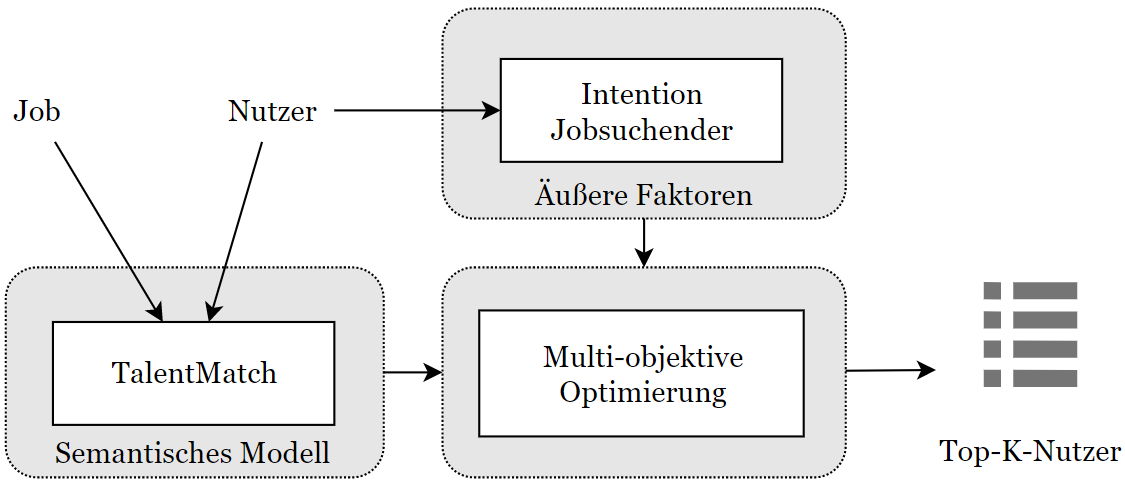
\includegraphics[width=0.9\textwidth]{gfx/talentMatch.png}
	\caption[Ansatz für die Integration äußerer Merkmale in semantische Modelle]{Ansatz für die Integration äußerer Merkmale in semantische Modelle\\
    (Eigene Darstellung in Anlehnung an \cite[S. 12]{rodriguez:inproceedings})}
	\label{fig:relatedwork:abb1}
\end{figure}

Im Detail stellen die Autoren eine Erweiterung des bestehenden \textit{TalentMatch}-Systems des sozialen Netzwerks LinkedIn vor, welche neben des semantischen Matches \cite[S. 2]{jannach:2:inproceedings} zwischen einer Person und einem Job (Objective 1) zusätzlich die Offenheit einer Person für einen Jobwechsel (Objective 2) in die Empfehlungserstellung (Ranking) miteinbezieht.
Dabei gehen die Autoren davon aus, dass die beiden Ziele möglicherweise miteinander konkurrieren, d.h. dass eine Person, die am besten auf eine Jobbeschreibung zutrifft, möglicherweise nicht offen für eine neue Stelle ist.
\textcite[S. 12]{rodriguez:inproceedings} untersuchen in ihrer Arbeit, ob die Berücksichtigung der Neigung von Personen für offene Jobpositionen den Nutzen der Nutzer des Systems dennoch positiv beeinflusst.
Den Nutzen operationalisieren die Autoren als das Engagement zwischen Jobsuchenden und Anbietern von Jobpositionen \cite[S. 14]{rodriguez:inproceedings}, welche diese über Menge aktiver, passiver und inaktiver Nutzer in dem System messen.
Die Integration der Berücksichtigung in das semantische Modell führen \textcite[S. 15]{rodriguez:inproceedings} systematisch über ein Re-Ranking durch.
Dies realisieren die Autoren über folgende Verlust-Funktion $L$ \cite[S. 13]{rodriguez:inproceedings}:
\begin{equation}\label{eq30}
    L(\alpha ,\beta) = -g(f(Y, X, [\alpha , \beta])) + \lambda \Delta (\pi (Y), \pi (f(Y,X,[\alpha ,\beta])))
\end{equation}
Nach \textcite[S. 15]{rodriguez:inproceedings} gibt Funktion $g$ die durchschnittliche Anzahl aktiver und passiver Nutzer in dem erweiterten System $f(Y, X, [\alpha , \beta])$ aus und $\Delta$ die Abweichung des Rankings $\pi (f(Y,X,[\alpha ,\beta]))$ des erweiterten Systems von dem Ranking $\pi (Y)$ des ursprünglichen semantischen Modells.
$\lambda$ stellt einen positiven Trade-Off-Parameter dar \cite[S. 13]{rodriguez:inproceedings}.
% \textcite[S. 13]{rodriguez:inproceedings} merken an, dass die Verlust-Funktion auch als Maximierungsproblem der Funktion $g$ dargestellt werden kann, welches $\Delta$ durch das Aufstellen einer Bedingung $c$ (d.h. $\Delta (\pi (Y), \pi (f(Y,X,[\alpha ,\beta]))) \leq c$) begrenzen kann.
Die Anpassung eines semantischen Matches $y$ realisieren \textcite[S. 15]{rodriguez:inproceedings} durch einen sogenannten "Boost", wobei zwischen einem Boost für aktive ($\alpha$) und passive ($\beta$) Nutzer unterschieden wird:
\begin{equation}\label{eq31}
    f(y,x,[\alpha ,\beta]) = y \cdot (\alpha^{1\{{x == \textnormal{active}\}}}) \cdot (\beta^{1\{{x == \textnormal{active}\}}})
\end{equation}
Hierbei ist $1\{x == \textnormal{active}\}$ gleich $1$, wenn die Bedingung innerhalb der geschweiften Klammer wahr ist und $0$ andernfalls.
Das Optimieren der Parameter $\alpha$ und $\beta$ führen \textcite[S. 15]{rodriguez:inproceedings} über eine Rastersuche durch.

\textcite[S. 15f.]{rodriguez:inproceedings} prüften ihren Ansatz anhand von 760 offenen Jobangeboten, von denen jedes zwischen 6 und 9000 mal in Empfehlungen auftauchte.
Dabei stellten die Autoren fest, dass eine signifikante Verbesserung des Nutzens mit einer akzeptablen und vorhersebaren Verschlechterung der semantischen Matches erreicht werden konnte \cite[S. 11]{rodriguez:inproceedings}.
% Dabei stellten die Autoren fest, dass bis zu einem gewissen Wert für Delta ein linearer Zusammenhang zwischen dem Zugewinn an durchschnittlich aktiven und passiven Nutzern und der Aufgabe von Übereinstimmung der Rankings besteht \cite[S. 16]{rodriguez:inproceedings}.
% Für bestimmte Kombinationen von $\alpha$ und $\beta$ konnte die Anzahl aktiver und passiver Nutzer in dem Top-K-Ranking durch Anwendung des erweiterten Modells verdoppelt werden, ohne massive Einbußen in den semantischen Matches einzufahren.
Kritisch betrachten \textcite[S. 16]{rodriguez:inproceedings} an ihrem Ansatz, dass für die Wirksamkeit eines Modells im praktischen Einsatz überprüft werden muss, ob die durchschnittliche Anzahl aktiver und passiver Nutzer tatsächlich repräsentativ für das Engagement von Nutzern in einem System ist.

\textcite[S. 1467ff.]{yildirim:article} stellen ebenfalls einen multi-objektiven Ansatz für wechselseitige Empfehlungssysteme im Online-Recruting vor.
Jedoch liegt der Fokus der Autoren auf der Entwicklung eines Modells für die Vorhersage der Reziprozität zwischen Jobkandidat und Recruiter (d.h. Jobpositon).
Reziprozität definieren \textcite[S. 1470]{yildirim:article} in ihrem Modell als die Wahrscheinlichkeit der Bewerbung eines Kandidats für eine Jobposition und die Wahrscheinlichkeit einer Kontaktaufnahme eines Recrutiers mit diesem Kandidat.
Hierbei betrachten die Autoren die Präferenzen separat als die beiden Outputs des Modells (daher multi-objektiv).
Die anschließende Kombination der beiden Wahrscheinlichkeit lassen die Autoren vorerst offen \cite[S. 1474]{yildirim:article}.
Sie gehen lediglich davon aus, dass dem Interesse eines Unternehmen bei der Jobauswahl höhere Bedeutung zukommt als dem Interesse eines Jobsuchenden.
Dies begründen die Autoren damit, dass Unternehmen die finale Entscheidung für bzw. gegen die Einstellung eines Kandidaten treffen \cite[S. 1470]{yildirim:article}.

\textcite[S. 705ff.]{kumari:article} setzen das multi-objektive Modell von \textcite[S. 1467ff.]{yildirim:article} als Benchmark für ihren Ansatz zu \ac{RRS} in Online-Dating-Plattformen ein.
Für die Kombination der unilateralen Präferenzen verwenden die Autoren das harmonische Mittel.
Dies begründen \textcite[S. 724]{kumari:article} damit, dass das harmonische Mittel kleinere Werte einer Datenreihe stärker berücksichtigt und dadurch die Interessen beider Parteien stärker vertreten sind als bei vergleichbaren Aggregationsmethoden.

Einen Vergleich verschiedener Aggregationsmethoden von Präferenzen in wechselseitigen Empfehlungssystemen führen \textcite[S. 4031ff.]{neve:inproceedings} und \textcite[S. 1ff.]{kumari:2:inproceedings} an.
\textcite[S. 4031ff.]{neve:inproceedings} vergleichen die Performance eines wechselseitigen Empfehlungssystems anhand der drei Pythagoras-Mittelwerte (arithmetisches, geometrisches und harmonisches Mittel) sowie der Cross-Ratio-Uninorm.
Die Cross-Ratio-Uni\-norm aggregiert zwei Werte $x$ und $y$ wie folgt \cite[S. 19]{appel:article}:
\begin{equation}\label{eq35}
    rcS(x,y) =
        \begin{cases}
            0 & \textnormal{wenn } (x,y) \in \{(0,1),(1,0)\} \\
            \frac{xy}{xy + (1-x) (1-y)} & \textnormal{sonst } \\
        \end{cases}
\end{equation}
Für den Vergleich der Aggregationsmethoden verwenden \textcite[S. 4034]{neve:inproceedings} die Performance-Metriken Precision, Recall und F1-Maß.
Dabei stellen die Autoren fest, dass das harmonische Mittel und die Cross-Ratio-Uninorm zu mehrheitlich höherer Precision führte als die anderen Methoden, wobei sie Precision (d.h. das Verhältnis relevanter Elemente zu allen empfohlenen Elementen) als besonders wichtiges Maß in \ac{RRS} bezeichnen \cite[S. 4035]{neve:inproceedings}.
Übergreifend konnte die Cross-Ratio-Uninorm die besten Performance-Ergebnisse erzielen \cite[S. 4035]{neve:inproceedings}.

\textcite[S. 4031]{neve:inproceedings} erkennen in ihrer Publikation die entscheidene Rolle der Kombination der Präferenzen der Parteien in wechselseitigen Empfehlungssystemen.
Aus den Ergebnissen ihres Experiments schließen die Autoren, dass wechselseitige Empfehlungssysteme durchaus von komplexeren Aggregationsfunktionen für die Kombination der Präferenzen profitieren könnten.
Daher argumentieren sie, dass Entscheidungen über die Aggregationsfunktion der Präferenzen in Algorithmen wechselseitiger Empfehlungssysteme zukünftig evidenzbasiert erfolgen sollen \cite[S. 4032]{neve:inproceedings}.
Weiter erkennen die Autoren den multi-kriteriellen Charakter der Thematik und schlagen die Verwendung von \ac{MCDA} (z.B. gewichtete Aggregationsmethoden \cite[S. 4036]{neve:inproceedings}) für die Kombination der unilateralen Präferenzen vor.

Zusätzlich zu den von \textcite[S. 4031ff.]{neve:inproceedings} angeführten Methoden betrachten \textcite[S. 1ff.]{kumari:2:inproceedings} das Produkt, den Schnitt und die Summe der unilateralen Präferenzen in ihrer Evaluation.
Aus der Publikation geht hervor, dass harmonisches Mittel, Cross-Ratio-Uninorm und Schnitt die besten Ergebnisse erzielen konnten.
Im Vergleich zu \textcite[S. 4031ff.]{neve:inproceedings} konnten in dem Versuch von \textcite[S. 5]{kumari:2:inproceedings} mit dem harmonischen Mittel als Aggregationsmethode die besten Ergebnisse erzielt werden.

\textcite[S. 41f.]{palomares:article} weisen in ihrer Veröffentlichung zum Stand der Forschung von wechselseitigen Empfehlungssystemen zuletzt ebenfalls auf die Bedeutung der Methodik für die Kombination unilateraler Präferenzen in ein bilaterales Resultat hin.
Darüber hinaus deuten nach \textcite[S. 42]{palomares:article} die Ergebnisse der Studie von \textcite[S. 4031ff.]{neve:inproceedings} darauf hin, dass eine Durchführung von Untersuchungen neuer Aggregationsfunktionen in bestehenden Modellen zu neuen Performance-Erkenntnissen führen kann.
% Weiterer Proof für bedeutsamkeit der aggregation unilateraler Präferenzen siehe hier: S. 41ff. : https://sci-hub.st/https://doi.org/10.1016/j.inffus.2020.12.001

% Das beschreibt den Anwendungsfall sehr gut: file://wsl%24/Ubuntu/home/masc6/Projects/masterarbeit/literatur/Utility-Based_Multi-Stakeholder_Recommendations_by_Multi-Objective_Optimization.pdf
% Das hier auch: file://wsl%24/Ubuntu/home/masc6/Projects/masterarbeit/literatur/Personalized%20Educational%20Learning%20with%20multi-stakeholder%20optimizations.pdf , Ergänzung siehe hier: https://sci-hub.st/10.1007/s11257-021-09291-x mit Kritik

% \subsection{Multi-kriterielle Bewertungen in Empfehlungssystemen}
% Erfinder des aggregation Funktion approaches: file://wsl%24/Ubuntu/home/masc6/Projects/masterarbeit/literatur/New_Recommendation_Techniques_for_Multicriteria_Rating_Systems.pdf
% Arbeit von Jannach wie hier beschrieben mit SVM: S. 102, file://wsl%24/Ubuntu/home/masc6/Projects/masterarbeit/literatur/E-Commerce.pdf
% multi-kriteria: Aggregation function approach: file://wsl%24/Ubuntu/home/masc6/Projects/masterarbeit/literatur/Recommending%20Hotels%20based%20on%20Multidimesional%20Customer%20Ratings.pdf
% ansatz von Tang: zusammenfügen mehrere feature bewertungen, sowie durchschnittsbewertung und kommentare, file:///C:/Users/masc6/Downloads/tdladmin,+TangandMcCalla_JoDI_final.pdf
% Slope one algorithmus und adaptive genetic algorithm von Hassan, S. 327, file://wsl%24/Ubuntu/home/masc6/Projects/masterarbeit/literatur/Imrpoving%20Prediction%20accuracy%20of%20multi-criteria%20recommender.pdf
% Liu et al.: Cluster von Nutzern, welche wichtigkeit einzelner Attribute angeben, zusammenfassung siehe hier S. 4, file:///C:/Users/masc6/Downloads/79_HDIOUD.pdf
% CCSD method, siehe: file:///C:/Users/masc6/Downloads/79_HDIOUD.pdf
% Wenn viele features: liwei et al (zsfsg. siehe hier: file://wsl%24/Ubuntu/home/masc6/Projects/masterarbeit/literatur/A%20Multi-criteria%20Recommender%20System%20Incorporating%20Intensity%20of%20Preferences.pdf )

% Darüber hinaus existieren einige Ansätze verwandter Domänen, die ebenfalls für die automatisierte Zuordnung von Personen für Jobpositionen relevant sind.
% Hier ggf. verwandte arbeiten in anderen domänen anführen. (z.B. Online Dating, Education)

% was gibt es also nicht? -> Reziprozität als gewichtetes Kriterium (Präferenz der empfohlenen Person zählt nicht genauso viel wie Präferenz des Nutzers, kann daher als gewichtetes Kriterium einer Aggregation Function betrachtet werden, welche über historische daten erlernt werden kann)
% Neue anwendungsbereiche von multi-kriteriellen EMpfehlungen in domänen wie online dating: zitat von S. 553, file://wsl%24/Ubuntu/home/masc6/Projects/masterarbeit/literatur/Towards%20the%20Next%20Generation%20of%20Multi-Criteria%20Recommender.pdf

% Zusätzlich: Darstellung negativer Präferenzen, siehe S. 288: https://link.springer.com/content/pdf/10.1007/978-3-642-22362-4.pdf?pdf=button
% -> RECON mit negativen Präferenzen

 \shorthandon{"}